\section{表达并行性}
我们已经知道如何在设备上放置代码(第 2 章)和数据(第 3 章)——我们现在要做的就是决定如何处理它。 
为此,我们现在转而填补一些迄今为止我们方便地遗漏或掩盖的事情。 
本章标志着从简单的教学示例到现实世界并行代码的转变,并扩展了我们在前面的章节中随意展示的代码示例的细节。

用一种新的并行语言编写我们的第一个程序似乎是一项艰巨的任务,特别是如果我们是并行编程的新手。 
语言规范不是为应用程序开发人员编写的,并且通常假设对术语有一定的熟悉; 它们不包含以下问题的答案:

\begin{itemize}
	\item 为什么有不止一种方式来表达并行性?

	\item 我应该使用哪种表达并行性的方法?

	\item 关于执行模型我到底需要了解多少?
\end{itemize}

本章旨在解决这些问题以及更多问题。 我们介绍了数据并行Kernel的概念,使用工作代码示例讨论了不同Kernel形式的优点和缺点,
并强调了Kernel执行模型的最重要方面。

\subsection{Kernel内的并行性}
近年来,并行Kernel作为表达数据并行性的强大手段而出现。 基于Kernel的方法的主要设计目标是跨各种设备的可移植性和高程序员生产力。 
因此,Kernel通常不会被硬编码为与特定数量或配置的硬件资源(例如,核心、硬件线程、SIMD [单指令,多数据]指令)一起工作。 
相反,Kernel根据抽象概念来描述并行性,然后实现(即编译器和运行时的组合)可以将其映射到特定目标设备上可用的硬件并行性。 
尽管此映射是实现定义的,但我们可以(并且应该)相信实现选择合理且能够有效利用硬件并行性的映射。

以与硬件无关的方式公开大量并行性可确保应用程序可以扩展(或缩小)以适应不同平台的功能,但是......

\begin{remark}
	保证功能便携性并不等于保证高性能!
\end{remark}

支持的设备存在很大的多样性,我们必须记住,不同的架构是针对不同的用例设计和优化的。 
每当我们希望在特定设备上实现最高水平的性能时,无论我们使用哪种编程语言,我们都应该始终期望需要一些额外的手动优化工作! 
此类特定于设备的优化的示例包括针对特定缓存大小的阻塞、选择分摊调度开销的工作粒度大小、
利用专用指令或硬件单元,以及最重要的是选择适当的算法。 其中一些示例将在第 15、16 和 17 章中重新讨论。

在应用程序开发过程中在性能、可移植性和生产力之间取得适当的平衡是我们所有人都必须面对的挑战,也是本书无法完全解决的挑战。 
然而,我们希望表明,带有 SYCL 的 C++ 提供了使用单一高级编程语言维护通用可移植代码和优化的目标特定代码所需的所有工具。 
剩下的就留给读者作为练习了!

\subsection{循环与Kernel}
迭代循环本质上是串行构造:循环的每次迭代都是按顺序执行的(即按顺序)。 
优化编译器也许能够确定循环的部分或全部迭代可以并行执行,
但它必须是保守的 - 如果编译器不够智能或没有足够的信息来证明并行执行始终是安全的,
则它 必须保留循环的顺序语义以确保正确性。

\begin{figure}[H]
	\centering
	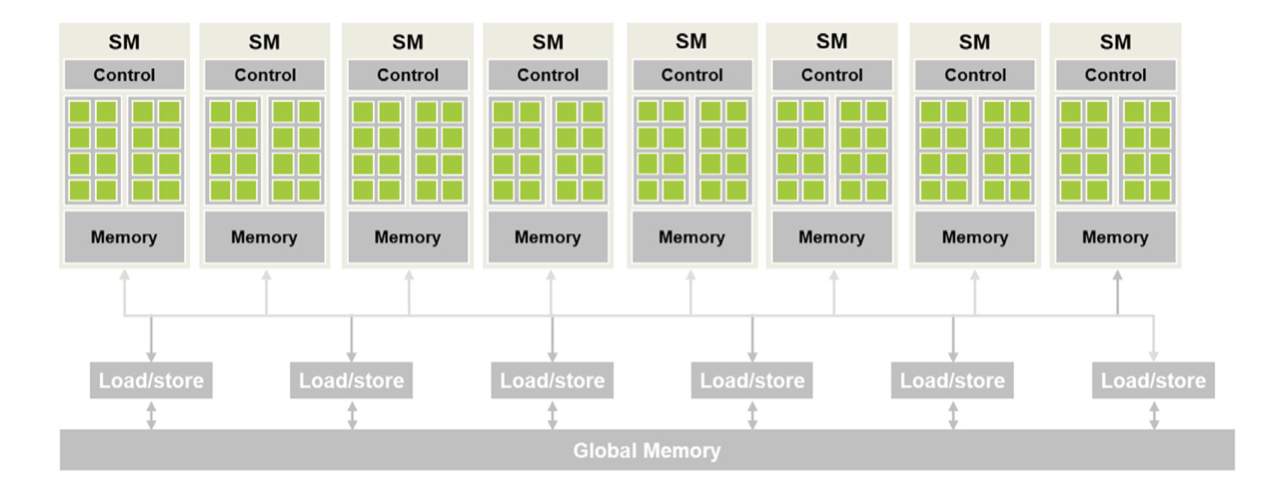
\includegraphics[width=0.9\textwidth]{figs/F4.1.png}
	\caption{\textit{将向量加法表示为串行循环}}
\end{figure}

考虑图 4-1 中的循环,它描述了一个简单的向量加法。 
即使在这样的简单情况下,证明循环可以并行执行也不是微不足道的:只有当 c 不与 a 或 b 重叠时,并行执行才是安全的,
而在一般情况下,如果没有运行时检查,就无法证明这一点! 为了解决这样的情况,语言添加了一些功能,
使我们能够为编译器提供额外的信息,
这些信息可以简化分析(例如,断言指针不与限制重叠)
或完全覆盖所有分析(例如,声明 循环是独立的或准确定义如何将循环调度到并行资源)。

并行循环的确切含义有些模糊(由于不同并行编程语言和运行时对该术语的重载),
但许多常见的并行循环结构表示应用于顺序循环的编译器转换。 这种编程模型使我们能够编写顺序循环,
然后才提供有关如何安全地并行执行不同迭代的信息。 
这些模型非常强大,与其他最先进的编译器优化集成良好,并极大地简化了并行编程,
但并不总是鼓励我们在开发的早期阶段考虑并行性。

并行Kernel不是循环并且没有迭代。 相反,Kernel描述了单个操作,
该操作可以多次实例化并应用于不同的输入数据; 当并行启动Kernel时,该操作的多个实例可能会同时执行。

\begin{figure}[H]
	\centering
	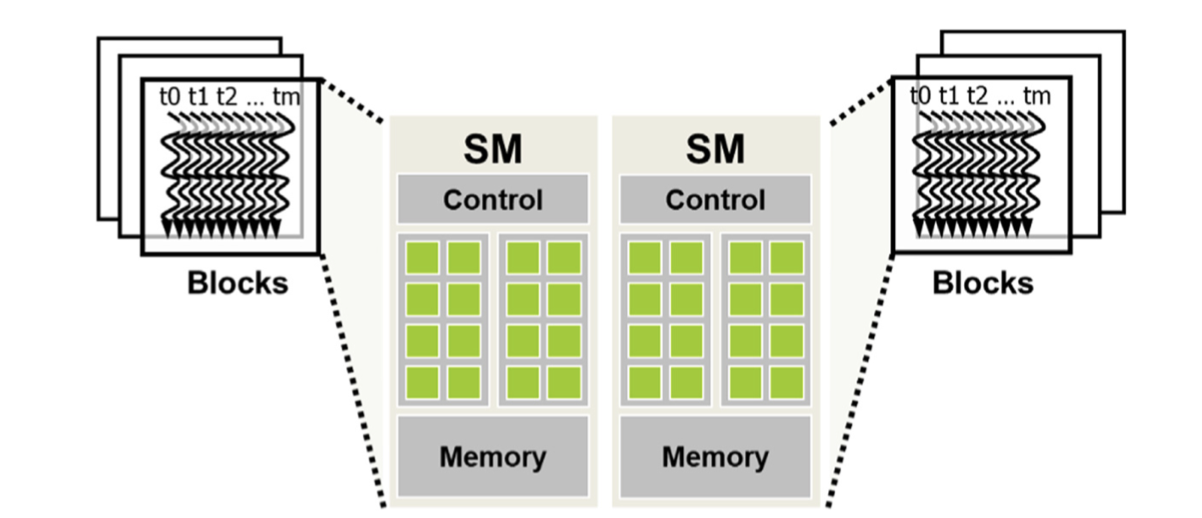
\includegraphics[width=0.9\textwidth]{figs/F4.2.png}
	\caption{\textit{循环重写(在伪代码中)为并行Kernel}}
\end{figure}

图 4-2 显示了使用伪代码重写为Kernel的简单循环示例。 
该Kernel中的并行机会是清晰明确的:Kernel可以由任意数量的实例并行执行,并且每个实例独立地应用于单独的数据块。 
通过将此操作编写为Kernel,我们断言并行运行是安全的(并且理想情况下应该并行运行)。

简而言之,基于Kernel的编程不是一种将并行性改进到现有顺序代码中的方法,而是一种编写显式并行应用程序的方法。

\begin{remark}
	我们越早将思维从并行循环转移到Kernel,就越容易使用 C++ 和 SYCL 编写有效的并行程序。
\end{remark}

\subsection{多维Kernel}
许多其他语言的并行结构是一维的,将工作直接映射到相应的一维硬件资源(例如,硬件线程的数量)。 
SYCL 中的并行Kernel是一个比这更高级别的概念,它们的维度更能反映我们的代码通常试图解决的问题(在一维、二维或三维空间中)。

然而,我们必须记住,并行Kernel提供的多维索引为程序员提供了便利,可以在底层一维空间之上实现。 
了解这种映射的行为方式可能是某些优化(例如,调整内存访问模式)的重要部分。

一个重要的考虑因素是哪个维度是连续的或单位步幅(即,多维空间中的哪些位置在一维映射中彼此相邻)。 
SYCL 中与并行性相关的所有多维量都使用相同的约定:维度从 0 到 N-1 进行编号,其中维度 N-1 对应于连续维度。 
无论多维数量被写为列表(例如,在构造函数中)或类支持多个下标运算符,此编号都从左到右应用(从左侧的维度 0 开始)。 
此约定与标准 C++ 中多维数组的行为一致。

\begin{figure}[H]
	\centering
	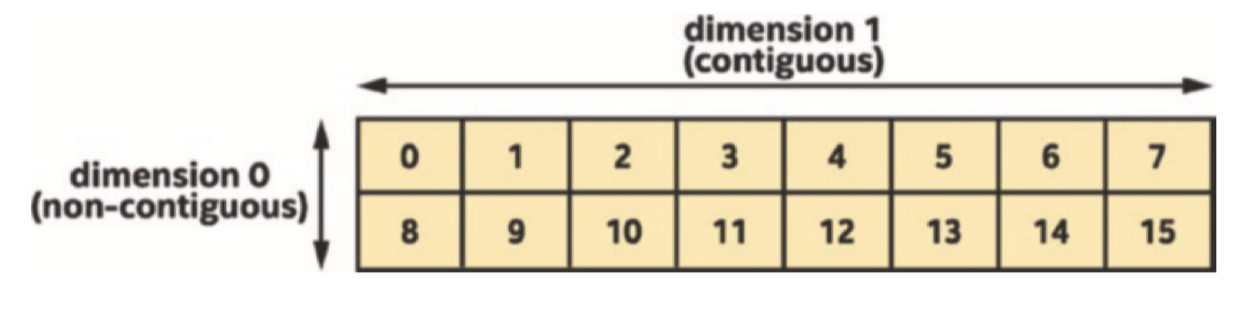
\includegraphics[width=0.9\textwidth]{figs/F4.3.png}
	\caption{\textit{映射到线性索引的大小 (2, 8) 的二维范围}}
\end{figure}

使用 SYCL 约定将二维空间映射到线性索引的示例如图 4-3 所示。 
我们当然可以自由地打破这个约定并采用我们自己的线性化索引的方法,
但必须小心行事——打破 SYCL 约定可能会对受益于 stride-one 访问的设备产生负面的性能影响。

如果应用程序需要三个以上的维度,我们必须负责使用模算术或其他技术手动在多维和线性索引之间进行映射。

\subsection{语言特性概述}
一旦我们决定编写并行Kernel,我们必须决定要启动什么类型的Kernel以及如何在程序中表示它。 
表达并行Kernel的方法有很多种,如果我们想掌握这门语言,我们需要熟悉每一种方法。

\subsubsection{将Kernel与主机代码分离}
我们有几种分离主机和设备代码的替代方法,可以在应用程序中混合和匹配这些代码:C++ lambda 表达式
或函数对象、通过互操作性接口定义的Kernel(例如 OpenCL C 源字符串)或二进制文件。 
其中一些选项已在第 2 章中介绍,其他选项将在第 10 章和第 20 章中详细介绍。

所有这些选项都共享表达并行性的基本概念。 为了保持一致性和简洁性,
本章中的所有代码示例都使用 C++ lambda 表达式来表达Kernel。

\begin{remark}[Lambda 表达式不被认为是有害的]
为了开始使用 SYCL,无需完全理解 C++ 规范中有关 lambda 表达式的所有内容 - 
我们需要知道的是 lambda 表达式的主体代表Kernel,并且(按值)捕获的变量将是 作为参数传递给Kernel。

使用 lambda 表达式而不是更详细的机制来定义Kernel不会对性能产生影响。 
支持 SYCL 的 C++ 编译器始终能够理解 lambda 表达式何时表示并行Kernel的主体,并可以相应地针对并行执行进行优化。

有关 C++ lambda 表达式的复习及其在 SYCL 中的使用说明,请参阅第 1 章。
有关使用 lambda 表达式定义Kernel的更多具体细节,请参阅第 10 章。
\end{remark}

\subsection{不同形式的并行Kernel}
SYCL中有三种不同的Kernel形式,支持不同的执行模型和语法。 
可以使用任何Kernel形式编写可移植Kernel,并且可以调整以任何形式编写的Kernel以在各种设备类型上实现高性能。 
然而,有时我们可能希望使用特定的形式来使特定的并行算法更容易表达或利用其他无法访问的语言功能。

第一种形式用于基本数据并行Kernel,并提供编写Kernel的最温和的介绍。 
对于基本Kernel,我们牺牲了对调度等低级功能的控制,以使Kernel的表达尽可能简单。 
各个Kernel实例如何映射到硬件资源完全由实现控制,因此随着基本Kernel复杂性的增加,推断其性能变得越来越困难。

第二种形式扩展了基本Kernel以提供对低级性能调整功能的访问。 
由于历史原因,第二种形式被称为 ND 范围(N 维范围)数据并行,最重要的是要记住,
它使某些Kernel实例能够分组在一起,从而允许我们对数据局部性和数据局部性进行一些控制。 
各个Kernel实例和用于执行它们的硬件资源之间的映射。

第三种形式提供了一种实验性的替代语法,用于使用类似于嵌套并行循环的语法来表达 ND 范围Kernel。 
第三种形式称为分层数据并行,指的是用户源代码中出现的嵌套结构的层次结构。 
编译器对此语法的支持仍然不成熟,并且许多 SYCL 实现不能像其他两种形式那样有效地实现分层数据并行Kernel。 
语法也不完整,因为 SYCL 有许多与分层Kernel不兼容或无法访问的性能支持功能。 
SYCL 中的分层并行性正在更新过程中,并且 SYCL 规范包含一条注释,建议新代码在该功能准备就绪之前不要使用分层并行性; 
为了与本说明的精神保持一致,本书的其余部分仅教授基本的和 ND 范围的并行性。

在更详细地讨论了不同Kernel形式的特性后,我们将在本章末尾再次讨论如何在不同Kernel形式之间进行选择。

\subsection{基础数据并行Kernel}
并行Kernel的最基本形式适用于高度并行的操作(即可以完全独立且以任何顺序应用于每条数据的操作)。 
通过使用这种形式,我们可以实现对工作安排的完全控制。 
因此,它是描述性编程构造的一个示例——我们描述操作是极其并行的,并且所有调度决策都是由实现做出的。

基本数据并行Kernel以单程序、多数据 (SPMD) 风格编写——单个“程序”(Kernel)应用于多条数据。 
请注意,由于数据相关的分支,此编程模型仍然允许Kernel的每个实例在代码中采用不同的路径。

SPMD 编程模型的最大优势之一是它允许将相同的“程序”映射到多个级别和类型的并行性,而无需我们的任何明确指示。 
同一程序的实例可以通过管道传输、打包在一起并使用 SIMD 指令执行、分布在多个硬件线程上或三者的混合。

\subsubsection{了解基本数据并行Kernel}
\begin{figure}[H]
	\centering
	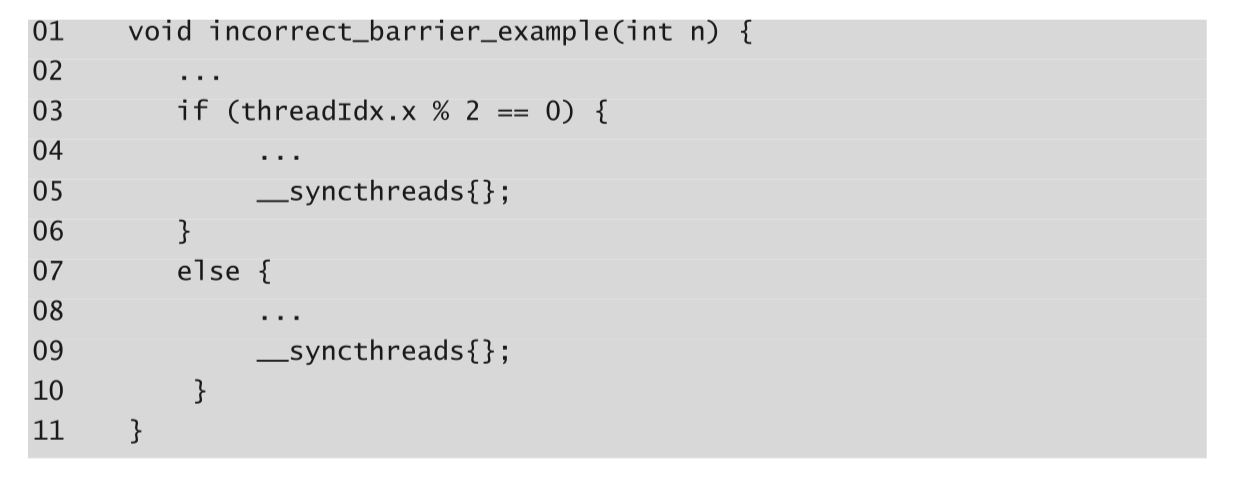
\includegraphics[width=0.9\textwidth]{figs/F4.4.png}
	\caption{\textit{基本并行Kernel的执行空间,显示为 64 个“项”的 2D 范围}}
\end{figure}

基本并行Kernel的执行空间被称为它的执行范围,并且Kernel的每个实例被称为一个“项”。 图 4-4 对此进行了示意性表示。

基本数据并行Kernel的执行模型非常简单:它允许完全并行执行,但不保证或要求它。 
“项”可以按任何顺序执行,包括在单个硬件线程上顺序执行(即,没有任何并行性)! 
因此,假设所有“项”都将并行执行的Kernel(例如,通过尝试同步“项”)可能很容易导致程序在某些设备上挂起。

然而,为了保证正确性,我们必须始终在假设Kernel可以并行执行的情况下编写Kernel。 
例如,我们有责任确保对内存的并发访问受到原子内存操作(参见第 19 章)的适当保护,以防止竞争条件。

\subsubsection{编写基本数据并行Kernel}
\begin{figure}[H]
	\centering
	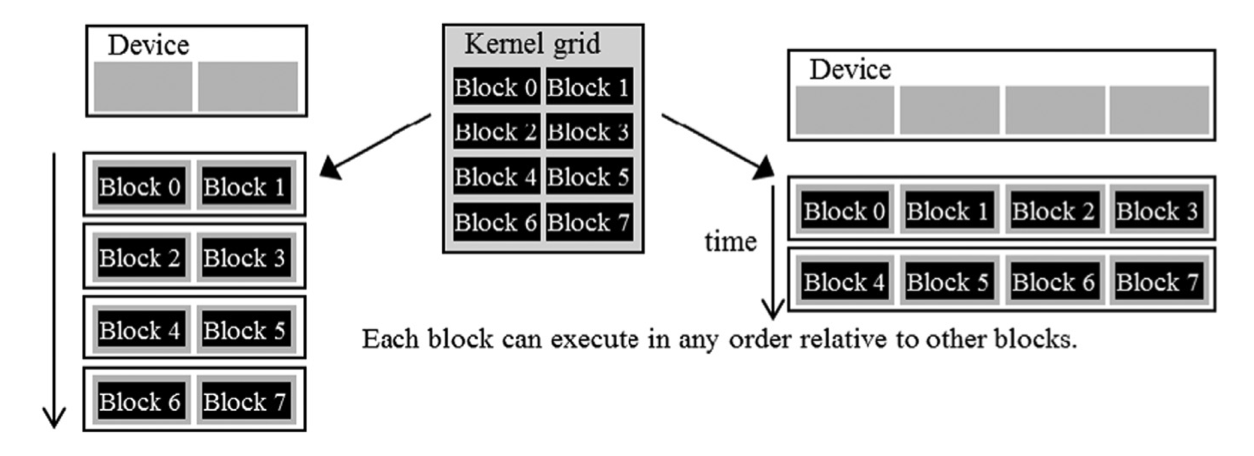
\includegraphics[width=0.9\textwidth]{figs/F4.5.png}
	\caption{\textit{用 parallel\_for 表达向量加法核}}
\end{figure}

基本数据并行Kernel使用parallel\_for 函数表示。 
图 4-5 显示了如何使用这个函数来表达向量加法,这是我们对“Hello, world!”的看法。 用于并行加速器编程。

该函数仅接受两个参数:第一个是范围(或整数),指定在每个维度中启动的“项”数,
第二个是要对该范围中的每个索引执行的Kernel函数。 
有几个不同的类可以被接受作为Kernel函数的参数,并且应该使用哪个类取决于哪个类公开所需的功能 - 我们稍后将重新讨论这一点。

\begin{figure}[H]
	\centering
	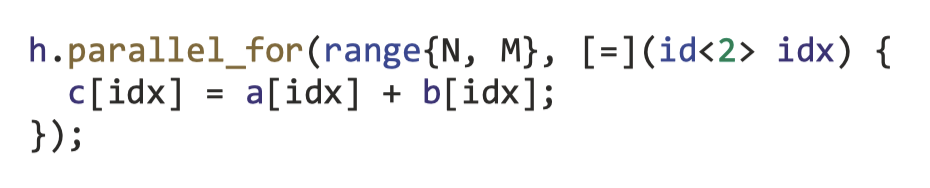
\includegraphics[width=0.9\textwidth]{figs/F4.6.png}
	\caption{\textit{用 parallel\_for 表达矩阵加法核}}
\end{figure}

图 4-6 显示了使用该函数非常类似地表达矩阵加法,除了二维数据之外,它与向量加法(在数学上)相同。 
这由Kernel反映出来——两个代码片段之间的唯一区别是所使用的 range 和 id 类的维度! 
可以用这种方式编写代码,因为 SYCL 访问器可以通过多维 id 进行索引。 
尽管看起来很奇怪,但它非常强大,使我们能够编写根据数据维度模板化的通用Kernel。

在C/C++中更常见的是使用多个索引和多个下标运算符来索引多维数据结构,并且访问器也支持这种显式索引。 
当Kernel同时操作不同维度的数据时,或者当Kernel的内存访问模式比直接使用“项”的 id 描述的更复杂时,
以这种方式使用多个索引可以提高可读性。

\begin{figure}[H]
	\centering
	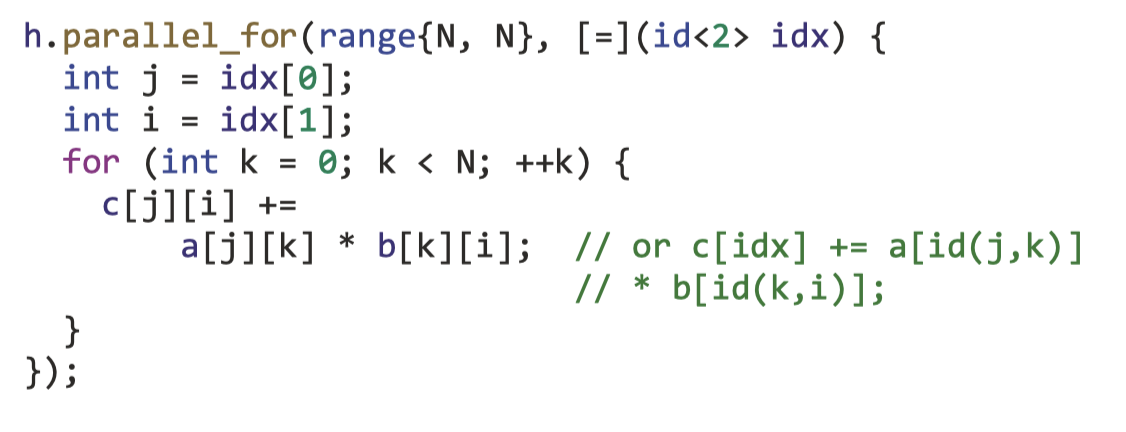
\includegraphics[width=0.9\textwidth]{figs/F4.7.png}
	\caption{\textit{用 parallel\_for 表达平方矩阵的朴素矩阵乘法核}}
\end{figure}

例如,图 4-7 中的矩阵乘法Kernel必须提取索引的两个单独分量,以便能够描述两个矩阵的行和列之间的点积。 
作者认为,一致使用多个下标运算符(例如,[j][k])比混合多种索引模式和构造二维 id 对象(例如 id(j,k))更具可读性,
但这是 只是个人喜好问题。

本章其余部分的示例都使用多个下标运算符,以确保所访问的缓冲区的维数不存在歧义。

\begin{figure}[H]
	\centering
	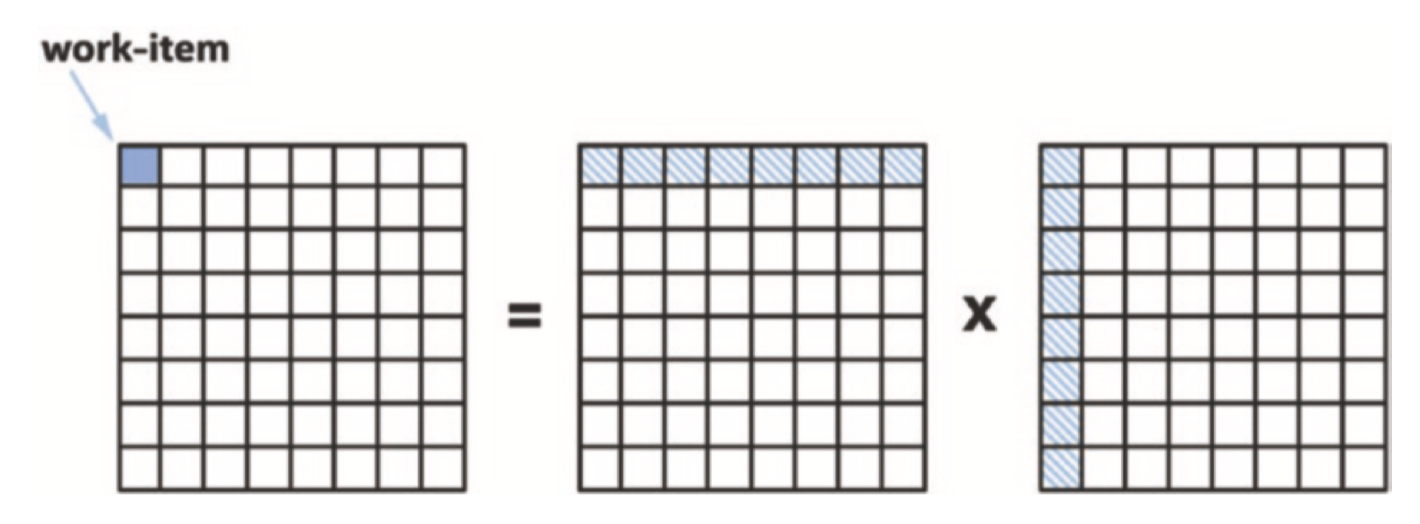
\includegraphics[width=0.9\textwidth]{figs/F4.8.png}
	\caption{\textit{将矩阵乘法工作映射到执行范围内的“项”}}
\end{figure}

图 4-8 中的图表显示了矩阵乘法Kernel中的工作如何映射到各个“项”。 
请注意,“项”数是根据输出范围的大小得出的,
并且多个“项”可以读取相同的输入值:每个“项”通过顺序迭代 C 矩阵的(连续)行来计算 C 矩阵的单个值。 
A 矩阵和 B 矩阵的一个(不连续)列。

\subsubsection{基本数据并行Kernel的详细信息}
基本数据并行Kernel的功能通过三个 C++ 类公开:range、id 和 item。 
我们已经在前面的章节中多次看到过 range 和 id 类,但我们在这里以不同的焦点重新审视它们。

\paragraph{range 类}

范围表示一维、二维或三维范围。 范围的维度是模板参数,因此必须在编译时已知,
但每个维度的大小是动态的,并在运行时传递给构造函数。 range 类的实例用于描述并行构造的执行范围和缓冲区的大小。

\begin{figure}[H]
	\centering
	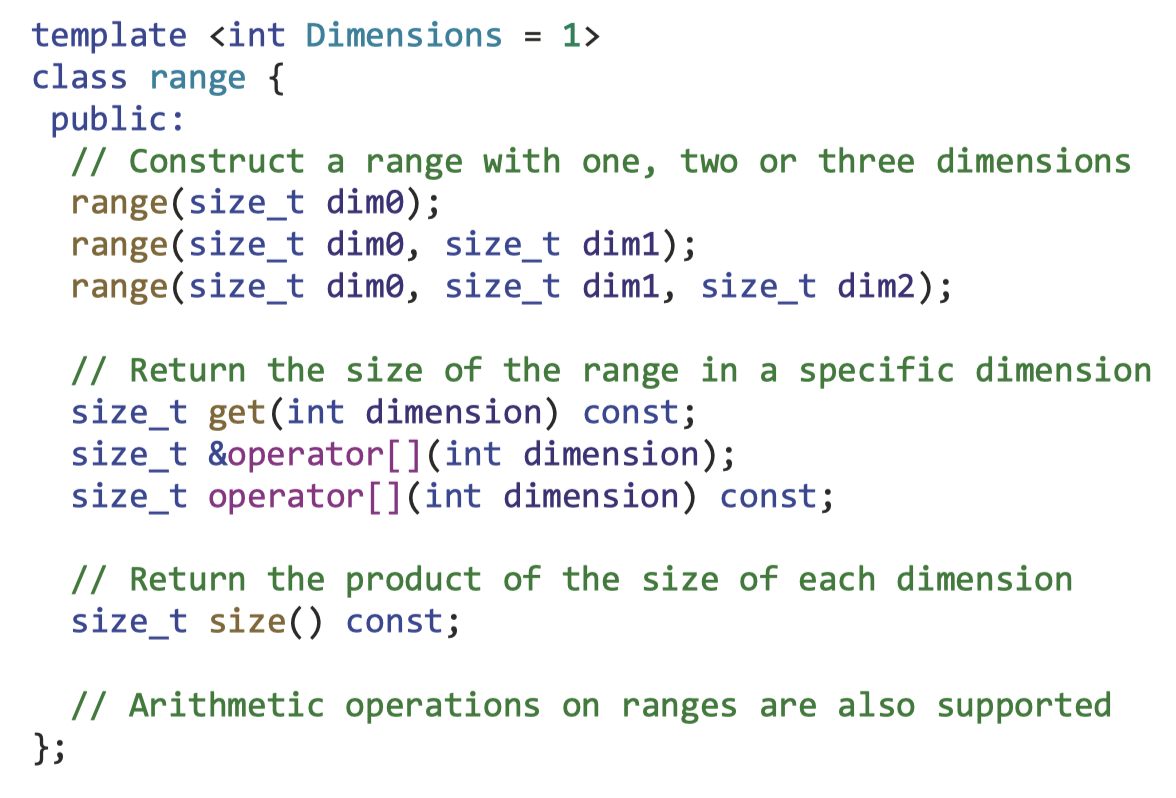
\includegraphics[width=0.9\textwidth]{figs/F4.9.png}
	\caption{\textit{range 类的简化定义}}
\end{figure}

图 4-9 显示了范围类的简化定义,显示了构造函数和查询其范围的各种方法。

\paragraph{id 类}

id 表示一维、二维或三维范围的索引。 
id 的定义在许多方面与 range 相似:它的维数也必须在编译时已知,
并且它可用于索引并行构造中Kernel的单个实例或缓冲区中的偏移量。

\begin{figure}[H]
	\centering
	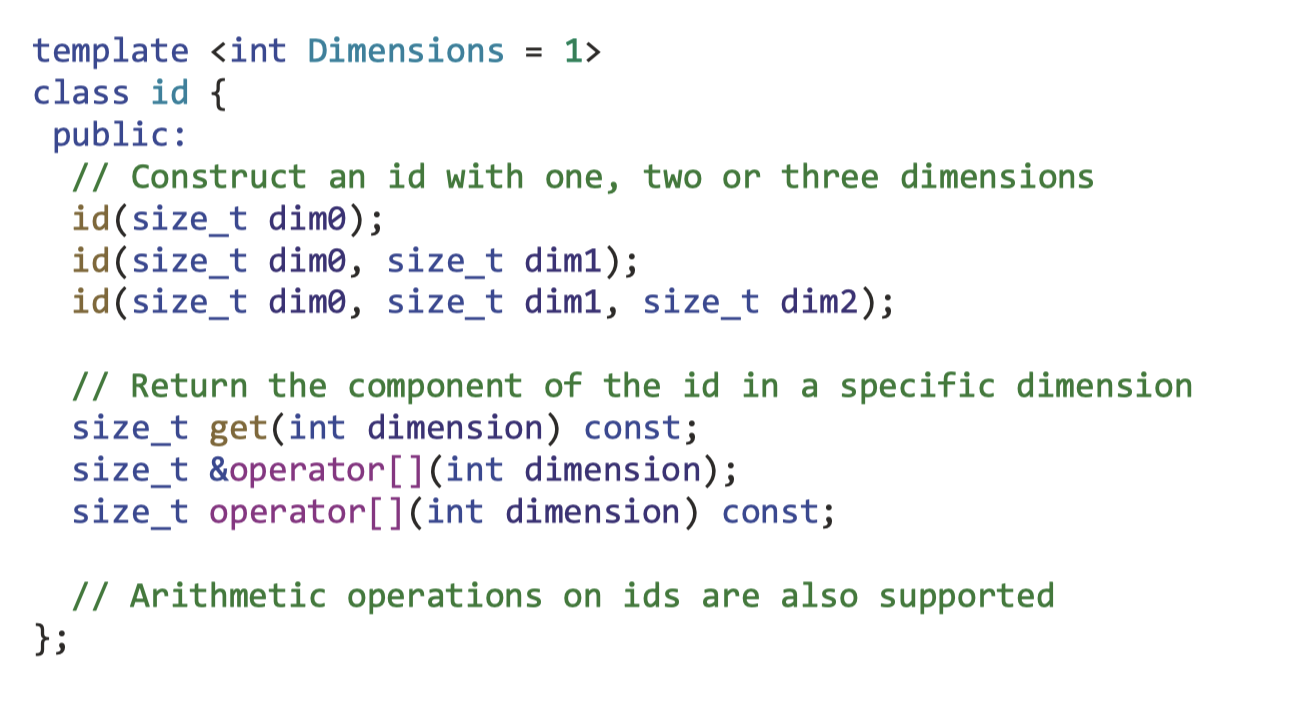
\includegraphics[width=0.9\textwidth]{figs/F4.10.png}
	\caption{\textit{id 类的简化定义}}
\end{figure}

如图 4-10 中 id 类的简化定义所示,id 在概念上只不过是一个、两个或三个整数的容器。 
我们可用的操作也非常简单:我们可以查询每个维度中索引的组成部分,并且可以执行简单的算术来计算新的索引。

虽然我们可以构造一个 id 来表示任意索引,但要获取与特定Kernel实例关联的 id,
我们必须接受它(或包含它的项)作为Kernel函数的参数。 
这个id(或者它的成员函数返回的值)必须被转发到我们想要查询索引的任何函数
——目前没有任何自由函数可以在程序中的任意点查询索引,但这可以简化为 SYCL 的未来版本。

每个接受 id 的Kernel实例只知道它被分配计算的范围内的索引,而对范围本身一无所知。 
如果我们希望Kernel实例知道它们自己的索引和范围,我们需要使用 item 类。

\paragraph{item 类}

“项” 代表Kernel函数的单个实例,封装了Kernel的执行范围和该范围内的实例索引(分别使用范围和 id)。 
与 range 和 id 一样,它的维数必须在编译时已知。

\begin{figure}[H]
	\centering
	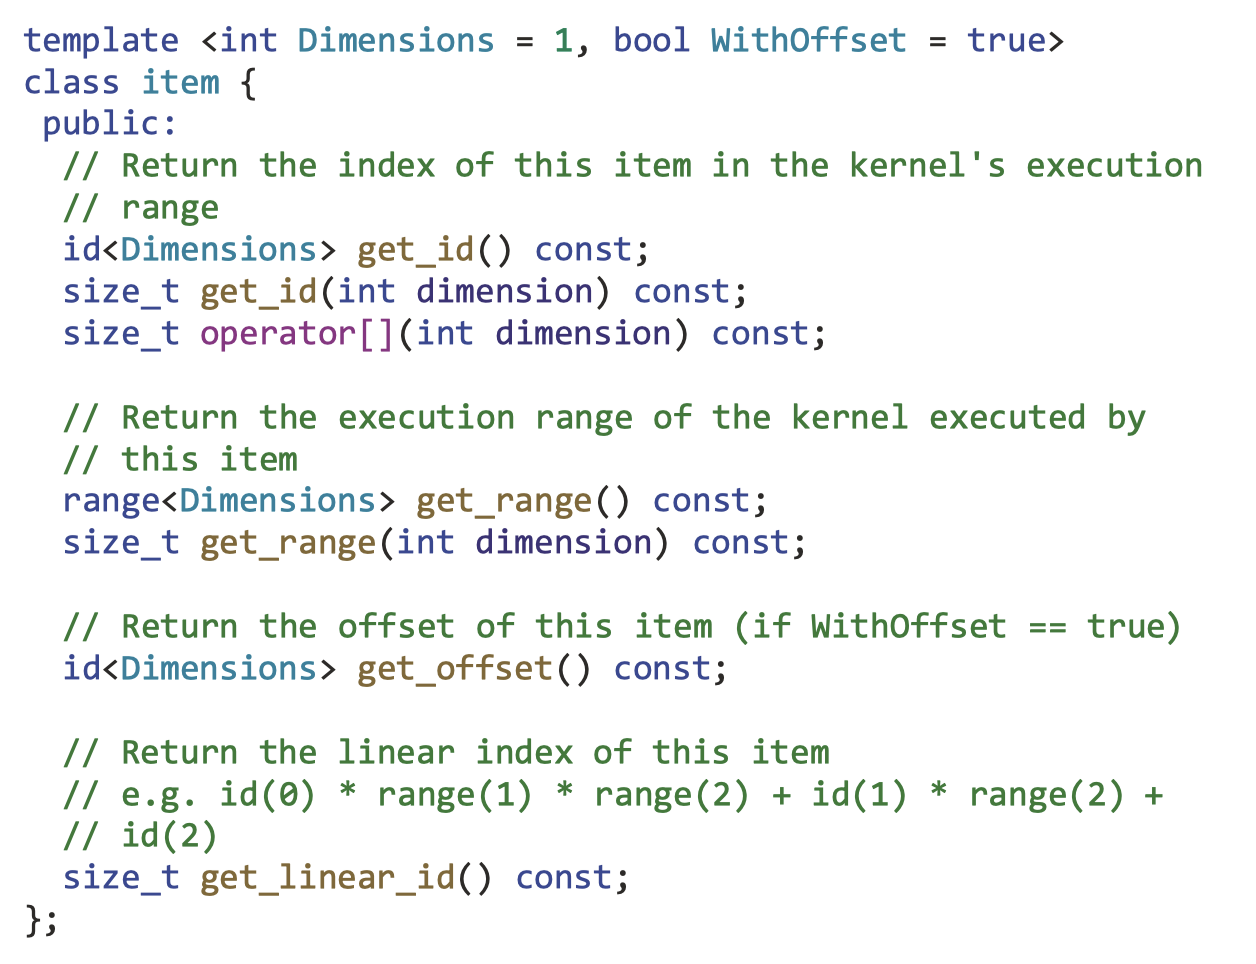
\includegraphics[width=0.9\textwidth]{figs/F4.11.png}
	\caption{\textit{item 类的简化定义}}
\end{figure}

图 4-11 给出了“项”类的简化定义。 
item 和 id 之间的主要区别在于 item 公开了额外的函数来查询执行范围的属性(例如,其大小)以及计算线性化索引的便利函数。 
与 id 一样,获取与特定Kernel实例关联的项的唯一方法是将其作为Kernel函数的参数接受。

\subsection{显式 ND 范围Kernel}
并行Kernel的第二种形式用“项”属于组的执行范围替换基本数据并行Kernel的平坦执行范围。 
这种形式最适合我们想要在Kernel中表达某些局部性概念的情况。 
为不同类型的组定义和保证不同的行为,使我们能够更深入地了解和/或控制如何将工作映射到特定的硬件平台。

因此,这些显式 ND 范围Kernel是更具规范性的并行构造的示例 - 我们规定了工作到每种类型组的映射,并且实现必须遵守该映射。 
然而,它并不完全是规定性的,因为组本身可以按任何顺序执行,并且实现对于每种类型的组如何映射到硬件资源保留了一定的自由度。 
这种规范性和描述性编程的结合使我们能够针对局部性设计和调整Kernel,而不会破坏其可移植性。

与基本数据并行Kernel一样,ND 范围Kernel以 SPMD 风格编写,
其中所有Work-Items都执行应用于多个数据的相同Kernel“程序”。 
主要区别在于每个程序实例都可以查询其在包含它的组中的位置,并且可以访问特定于每种类型的组的附加功能(请参见第 9 章)。

\subsubsection{了解显式 ND 范围并行Kernel}
ND范围Kernel的执行范围分为Work-Groups、Sub-Groups和Work-Items。 
ND-range 表示总的执行范围,它被划分为统一大小的Work-Groups
(即,Work-Groups大小必须在每个维度上精确地除以 ND-range 大小)。 
每个Work-Groups可以根据实施进一步划分为Sub-Groups。 
了解为Work-Items和每种类型的组定义的执行模型是编写正确且可移植的程序的重要组成部分。

\begin{figure}[H]
	\centering
	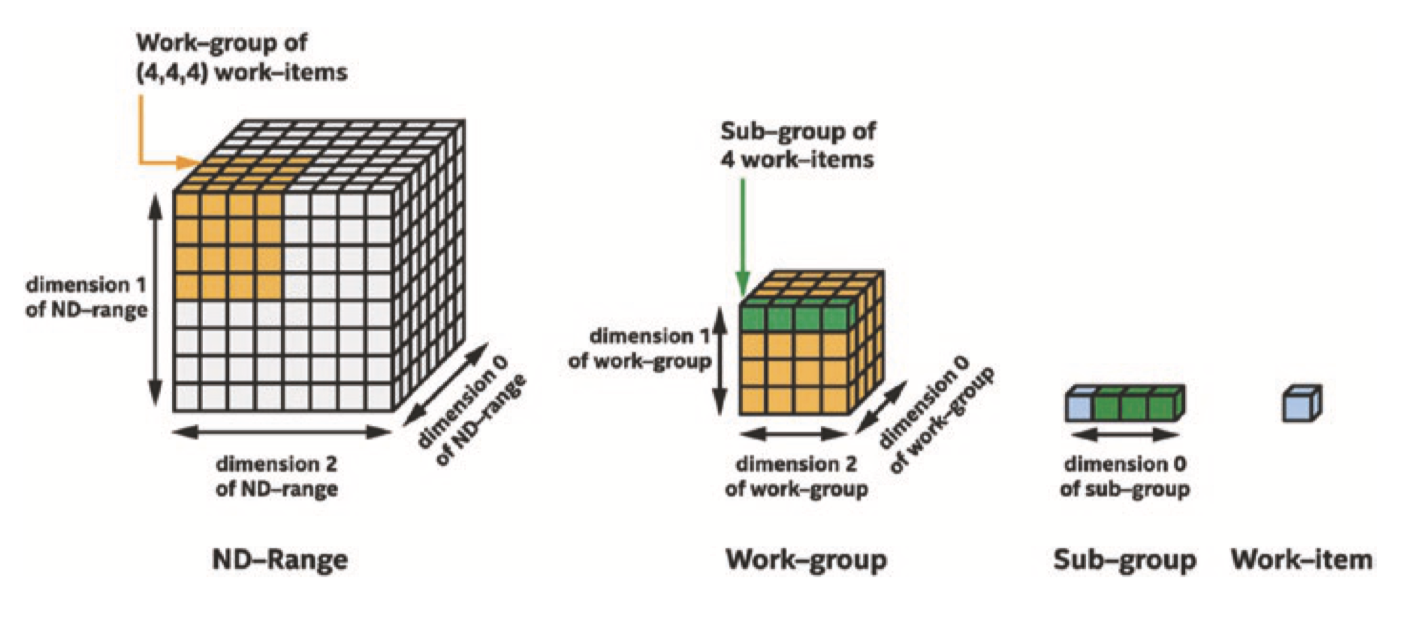
\includegraphics[width=0.9\textwidth]{figs/F4.12.png}
	\caption{\textit{三维 ND 范围分为Work-Groups、Sub-Groups和Work-Items}}
\end{figure}

图 4-12 显示了大小为 (8, 8, 8) 的 ND 范围分为 8 个大小为 (4, 4, 4) 的Work-Groups的示例。 
每个Work-Groups包含 16 个一维Sub-Groups,每组有 4 个Work-Items。 
请特别注意维度的编号:Sub-Groups始终是一维的,因此 ND 范围和Work-Groups的维度 2 成为Sub-Groups的维度 0。

从每种类型的组到硬件资源的精确映射是实现定义的,正是这种灵活性使得程序能够在各种硬件上执行。 
例如,Work-Items可以完全顺序执行、由硬件线程和/或SIMD指令并行执行、或者甚至由专门为Kernel配置的硬件管道执行。

在本章中,我们仅关注 ND 范围执行模型在通用目标平台方面的语义保证,并且我们不会涵盖其到任何一个平台的映射。 
有关 GPU、CPU 和 FPGA 的硬件映射和性能建议的详细信息,请分别参阅第 15、16 和 17 章。

\subsubsection{编写显式 ND 范围数据并行Kernel}
\paragraph{Work-Items}

Work-Items代表核函数的各个实例。 
在没有其他分组的情况下,Work-Items可以按任何顺序执行,并且不能相互通信或同步,
除非通过对全局内存的原子内存操作(参见第 19 章)。

\paragraph{Work-Groups}

ND 范围内的Work-Items被组织成Work-Groups。 Work-Groups可以按任何顺序执行,
不同Work-Groups中的Work-Items不能相互通信,
除非通过对全局内存的原子内存操作(参见第 19 章)。 
然而,当使用某些构造时,Work-Groups内的Work-Items具有一些调度保证,并且该局部性提供了一些附加功能:

\begin{enumerate}
	\item Work-Groups中的Work-Items可以访问Work-Groups本地内存,该内存可能会映射到某些设备上的专用快速内存(请参阅第 9 章)。

	\item Work-Groups中的Work-Items可以使用Work-GroupsBarrier进行同步,并使用Work-Groups内存栅栏保证内存一致性(参见第 9 章)。

	\item Work-Groups中的Work-Items可以访问组功能,提供通用通信例程(参见第 9 章)和组算法的实现,
	提供通用并行模式的实现,例如归约和扫描(参见第 14 章)。
\end{enumerate}

Work-Groups中Work-Items的数量通常在运行时为每个Kernel配置,
因为最佳分组将取决于可用并行度(即 ND 范围的大小)和目标设备的属性 。 
我们可以使用设备类的查询函数确定特定设备支持的每个Work-Groups的最大Work-Items数(参见第 12 章),
并且我们有责任确保每个Kernel请求的Work-Groups大小 已验证。

Work-Groups执行模型中有一些微妙之处值得强调。

首先,虽然Work-Groups中的Work-Items被调度到单个计算单元,
但是Work-Groups的数量和计算单元的数量之间不需要有任何关系。 
事实上,ND 范围内的Work-Groups数量可能比给定设备可以同时执行的Work-Groups数量大很多倍! 
我们可能会尝试编写通过依赖非常聪明的设备特定调度来跨Work-Groups同步的Kernel,
但我们强烈建议不要这样做——这样的Kernel今天可能可以工作,但不能保证它们将来也能工作 实现,
并且当移动到不同的设备时很可能会中断。

其次,虽然Work-Groups中的工作“项”被安排为可以相互合作,
但它们不需要提供任何具体的前进进度保证——在障碍和集体之间顺序执行Work-Groups内的工作“项”是一种 有效实施。 
仅当使用提供的Barrier和集合函数执行时,同一Work-Groups中的Work-Items之间的通信和同步才能保证安全,
并且手工编码的同步例程可能会死锁。

\begin{remark}[在Work-Groups中思考]
	Work-Groups在许多方面与其他编程模型中的任务概念相似(例如,线程构建块):任务可以按任何顺序执行(由调度程序控制);
	超额订阅带有任务的机器是可能的(甚至是可取的);
	尝试在一组任务中实现Barrier通常不是一个好主意(因为它可能非常昂贵或与调度程序不兼容)。
	如果我们已经熟悉了基于任务的编程模型,我们可能会发现将Work-Groups视为数据并行任务是有用的。
\end{remark}

\paragraph{Sub-Groups}

在许多现代硬件平台上,Work-Groups中的Work-Items子集(称为Sub-Groups)在附加调度保证的情况下执行。 
例如,Sub-Groups中的Work-Items可以由于编译器向量化而同时执行,和/或Sub-Groups本身可以以强大的前进进度保证来执行,
因为它们被映射到独立的硬件线程。

当使用单一平台时,很容易将关于这些执行模型的假设融入到我们的代码中,
但这使得它们本质上不安全且不可移植——在不同编译器之间移动时,甚至在不同代硬件之间移动时,它们可能会崩溃。 同一个供应商!

将Sub-Groups定义为语言的核心部分为我们提供了一种安全的替代方案,可以避免做出稍后可能被证明是特定于设备的假设。 
利用Sub-Groups功能还允许我们在低级别(即接近硬件)推理Work-Items的执行,并且是跨许多平台实现非常高的性能水平的关键。

与Work-Groups一样,Sub-Groups内的Work-Items可以同步、保证内存一致性或通过组函数和组算法执行常见的并行模式。 
然而,Sub-Groups没有Work-Groups本地存储器的等价物(即,没有Sub-Groups本地存储器)。 
相反,Sub-Groups中的Work-Items可以使用组算法的子集(俗称“SHUFFLE”操作)直接交换数据,无需显式内存操作(第 9 章)。

\begin{remark}[为什么是“SHUFFLE”?]
	OpenCl、CUDA 和 SPIR-V 等语言中的“shuffle”操作的名称中都包含“shuffle”(例如,sub\_group\_shuffle、
	\_\_shfl 和 OpGroupNonUniformShuffle)。SYCl 采用不同的命名约定,
	以避免与 C++ 中定义的 std::shuffle 函数混淆(该函数随机重新排序范围的内容)。
\end{remark}

Sub-Groups的某些方面是由实现定义的,不在我们的控制范围内。 
然而,对于给定的设备、Kernel和 ND 范围的组合,Sub-Groups具有固定(一维)大小,
我们可以使用Kernel类的查询函数来查询该大小(参见第 10 章和第 12 章) 。 
默认情况下,每个Sub-Groups的Work-Items数量也由实现选择 - 
我们可以通过在编译时请求特定的Sub-Groups大小来覆盖此行为,
但必须确保我们请求的Sub-Groups大小与设备兼容 。

与Work-Groups一样,Sub-Groups中的Work-Items不需要提供任何特定的前进进度保证 - 
实现可以自由地顺序执行Sub-Groups中的每个Work-Items,
并且仅在Work-Items发生变化时才在Work-Items之间切换。 遇到Sub-Groups集体函数。 
然而,在某些设备上,Work-Groups内的所有Sub-Groups都保证最终执行(取得进展),这是多种生产者-消费者模式的基石。 
这是当前实现定义的行为,因此如果我们希望Kernel保持可移植性,我们就不能依赖Sub-Groups来取得进展。 
我们期望 SYCL 的未来版本能够提供描述Sub-Groups进度保证的设备查询。

\begin{figure}[H]
	\centering
	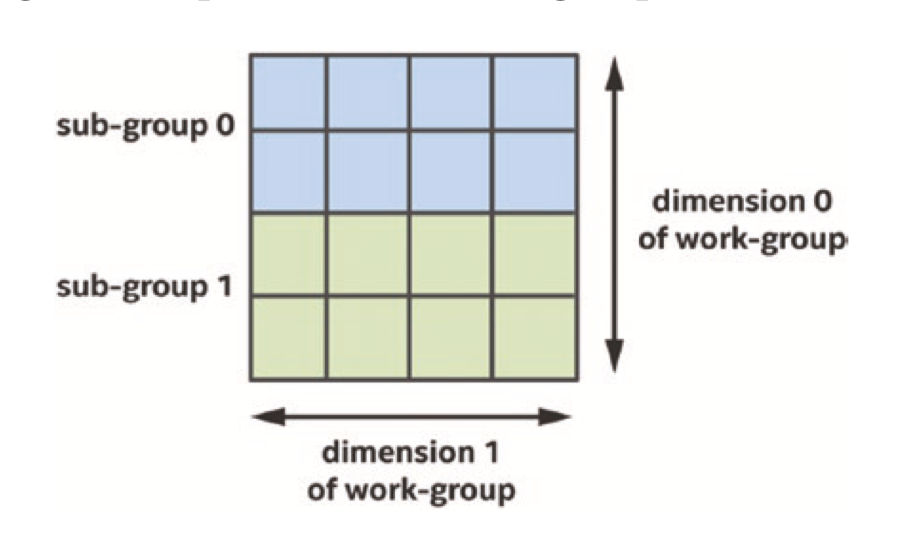
\includegraphics[width=0.9\textwidth]{figs/F4.13.png}
	\caption{\textit{一种可能的Sub-Groups映射,
	其中Sub-Groups大小允许大于Work-Groups的最高编号(连续)维度的范围,因此Sub-Groups看起来是“环绕”}}
\end{figure}


\begin{figure}[H]
	\centering
	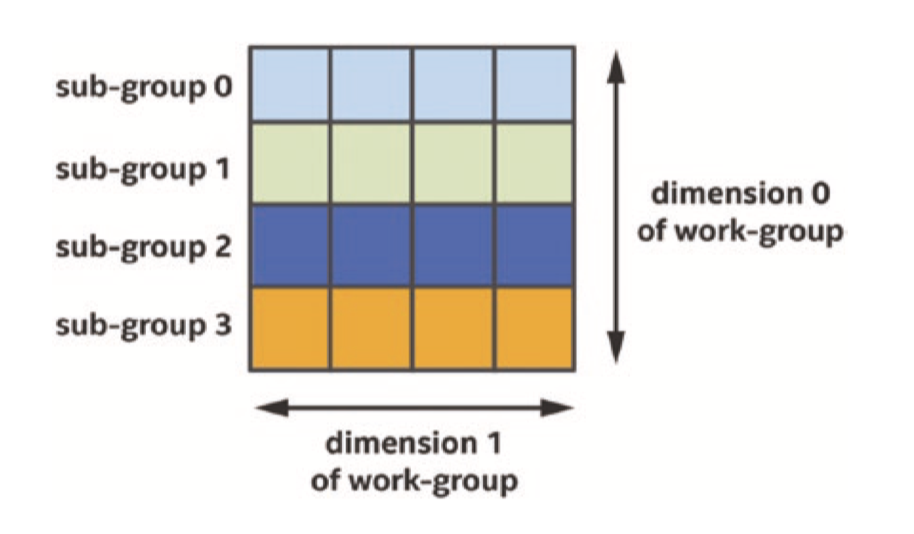
\includegraphics[width=0.9\textwidth]{figs/F4.14.png}
	\caption{\textit{另一种可能的Sub-Groups映射,
	其中Sub-Groups大小不允许大于Work-Groups的最高编号(连续)维度的范围}}
\end{figure}

当为特定设备编写Kernel时,Work-Items到Sub-Groups的映射是已知的,并且我们的代码通常可以利用此映射的属性来提高性能。 
然而,一个常见的错误是假设因为我们的代码可以在一台设备上运行,所以它也可以在所有设备上运行。 
图 4-13 和 4-14 仅显示了将范围为 {4, 4} 的多维Kernel中的Work-Items映射到Sub-Groups(最大Sub-Groups大小为 8)时的两种可能性。 
图 4-13 生成两个包含 8 个Work-Items的Sub-Groups,而图 4-14 中的映射生成四个包含 4 个Work-Items的Sub-Groups!

SYCL 当前不提供查询Work-Items如何映射到Sub-Groups的方法,也不提供请求特定映射的机制。 
使用Sub-Groups编写可移植代码的最佳方法是使用一维Work-Groups或多维Work-Groups,其中最高编号的维度可被Kernel所需的Sub-Groups大小整除。

\begin{remark}[在Sub-Groups中思考]
	如果我们来自一个需要我们考虑显式矢量化的编程模型,那么将每个Sub-Groups视为一组打包到 SIMD 寄存器中的Work-Items可能会很有用,
	其中Sub-Groups中的每个Work-Items对应于 SIMD 通道。当多个Sub-Groups同时飞行并且设备保证它们会向前推进时,
	这种心智模型扩展到将每个Sub-Groups视为并行执行的单独向量指令流。
\end{remark}

\paragraph{编写显式 ND 范围数据并行Kernel}

\begin{figure}[H]
	\centering
	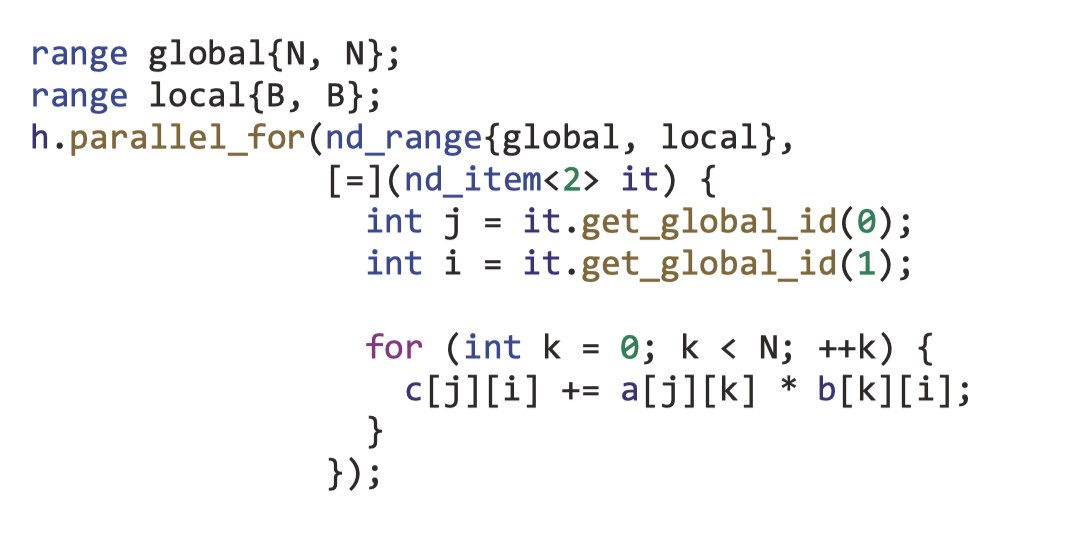
\includegraphics[width=0.9\textwidth]{figs/F4.15.png}
	\caption{\textit{用 ND 范围parallel\_for表达朴素矩阵乘法核}}
\end{figure}

\begin{figure}[H]
	\centering
	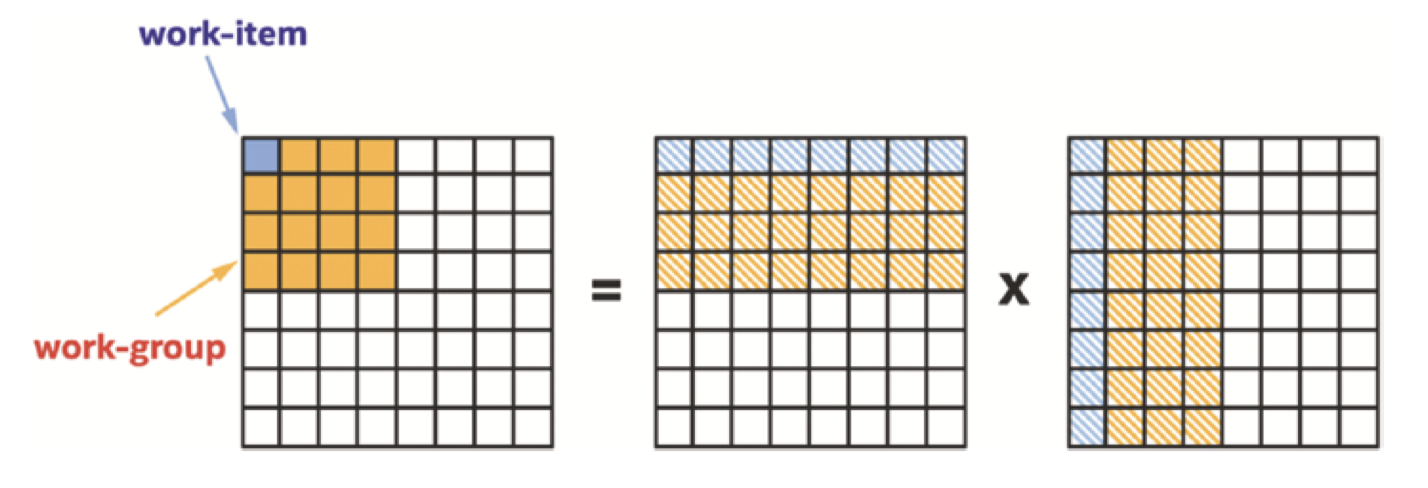
\includegraphics[width=0.9\textwidth]{figs/F4.16.png}
	\caption{\textit{将矩阵乘法映射到Work-Groups和Work-Items}}
\end{figure}

图 4-15 使用 ND 范围并行Kernel语法重新实现了我们之前看到的矩阵乘法Kernel,
图 4-16 中的图表显示了该Kernel中的工作如何映射到每个Work-Groups中的Work-Items。 
以这种方式对Work-Items进行分组可确保访问的局部性,并有望提高缓存命中率:
例如,图 4-16 中的Work-Groups的本地范围为 (4, 4),包含 16 个Work-Items,
但仅访问 4 个Work-Items 数据量是单个Work-Items的数据量的四倍——换句话说,我们从内存加载的每个值都可以重复使用四次。

到目前为止,我们的矩阵乘法示例依赖于硬件缓存来优化同一Work-Groups中的Work-Items对 A 和 B 矩阵的重复访问。 
此类硬件缓存在传统 CPU 架构上很常见,并且在 GPU 架构上变得越来越常见,
但一些架构已经明确管理可以提供更高性能(例如,通过更低延迟)的“暂存器”内存。 
ND 范围Kernel可以使用本地访问器来描述应放置在Work-Groups本地内存中的分配,
然后实现可以自由地将这些分配映射到特殊内存(如果存在)。 该Work-Groups本地内存的使用将在第 9 章中介绍。

\subsubsection{显式 ND 范围数据并行Kernel的详细信息}
与基本数据并行Kernel相比,ND 范围数据并行Kernel使用不同的类:range 被 nd\_range 替换,item 被 nd\_item 替换。 
还有两个新类,代表Work-Items可能所属的不同类型的组:与Work-Groups相关的功能封装在 group 类中,
与Sub-Groups相关的功能封装在 sub\_group 类中。

\paragraph{nd\_range 类}

nd\_range 使用 range 类的两个实例表示分组执行范围:一个表示全局执行范围,另一个表示每个Work-Groups的本地执行范围。 
图 4-17 给出了 nd\_range 类的简化定义。

\begin{figure}[H]
	\centering
	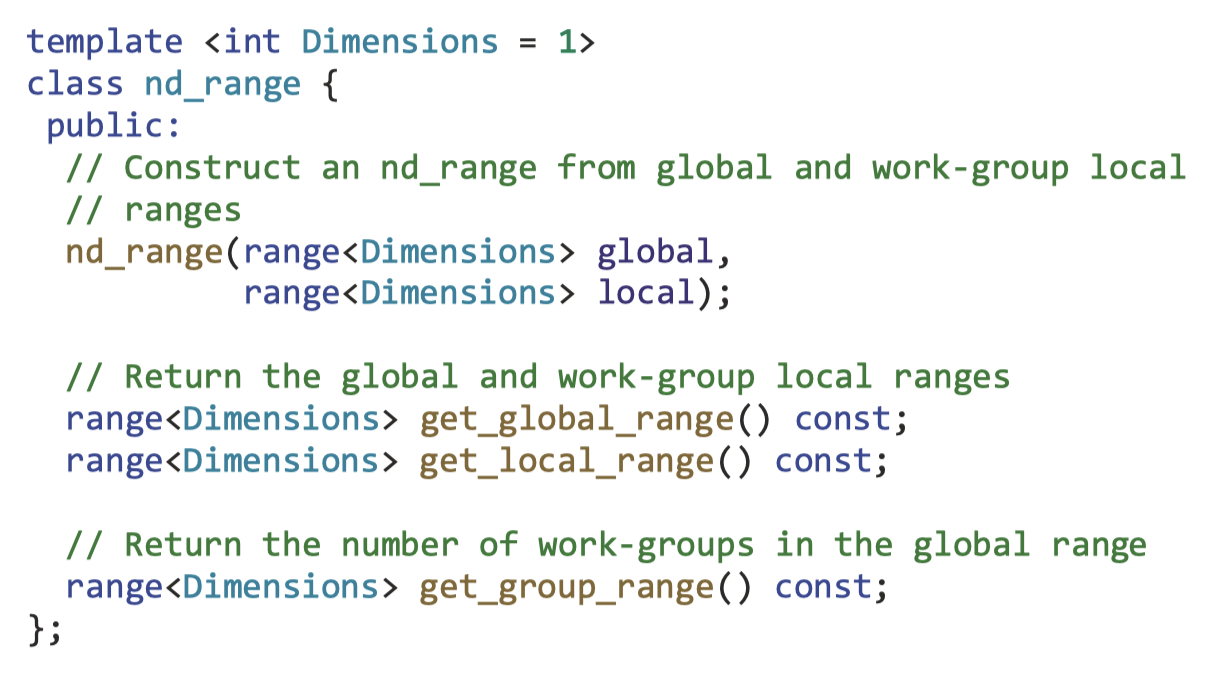
\includegraphics[width=0.9\textwidth]{figs/F4.17.png}
	\caption{\textit{nd\_range类的简化定义}}
\end{figure}

可能有点令人惊讶的是 nd\_range 类根本没有提及Sub-Groups:Sub-Groups范围在构造过程中没有指定并且无法查询。 
造成这一遗漏的原因有两个。 首先,Sub-Groups是一个低级实现细节,对于许多Kernel来说可以忽略。 
其次,有多种设备恰好支持一种有效的Sub-Groups大小,并且在任何地方指定该大小将是不必要的冗长。 
与Sub-Groups相关的所有功能都封装在一个专用类中,稍后将讨论该类。

\paragraph{nd\_item 类}

nd\_item 是“项”的 ND 范围形式,再次封装了Kernel的执行范围以及该范围内“项”的索引。 
nd\_item 与 item 的不同之处在于如何查询和表示其在范围中的位置,如图 4-18 中简化的类定义所示。 
例如,我们可以使用 get\_global\_id() 函数查询(全局)ND 范围中的“项”索引,
或者使用 get\_local\_id() 函数查询“项”在其(本地)父Work-Groups中的索引。

\begin{figure}[H]
	\centering
	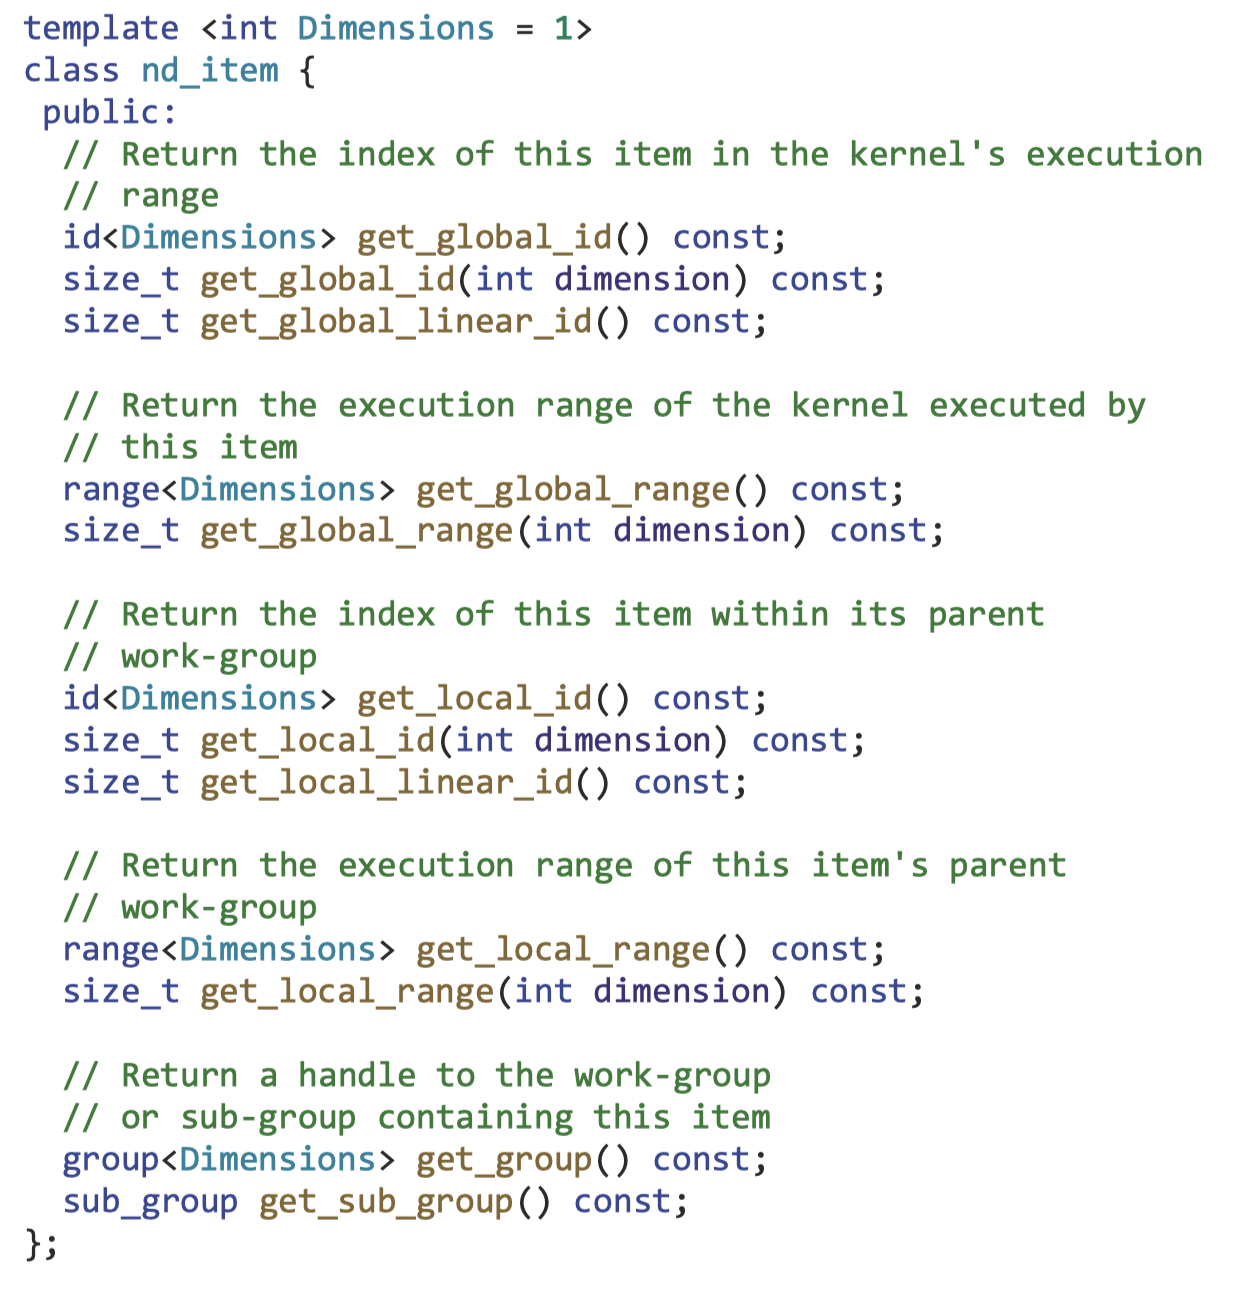
\includegraphics[width=0.9\textwidth]{figs/F4.18.png}
	\caption{\textit{nd\_item类的简化定义}}
\end{figure}

nd\_item 类还提供了用于获取描述“项”所属组和Sub-Groups的类句柄的函数。 
这些类提供了用于查询 ND 范围中“项”索引的替代接口。

\paragraph{group 类}

group 类封装了与Work-Groups相关的所有功能,简化的定义如图4-19所示。

\begin{figure}[H]
	\centering
	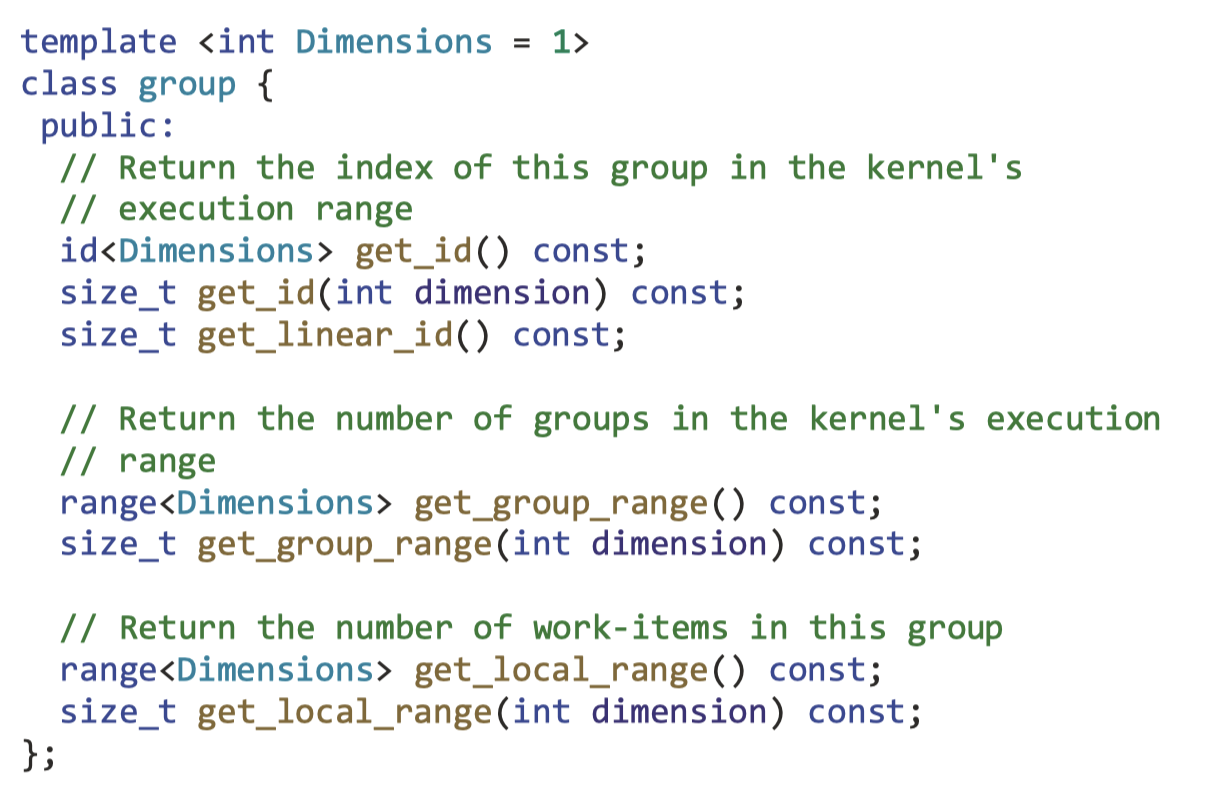
\includegraphics[width=0.9\textwidth]{figs/F4.19.png}
	\caption{\textit{group 类的简化定义}}
\end{figure}

group 类提供的许多函数在 nd\_item 类中都有等效的函数:
例如,调用 group.get\_group\_id() 相当于调用 item.get\_group\_id(),
调用 group.get\_local\_range() 相当于调用 item.get\_local\_range()。 
如果我们不使用任何 group 函数或算法,我们还应该使用 group 类吗? 
直接使用 nd\_item 中的函数而不是创建中间组对象不是更简单吗? 
这里有一个权衡:使用 group 需要我们编写稍微多一些的代码,但该代码可能更容易阅读。 
例如,考虑图 4-20 中的代码片段:很明显,body 期望被组中的所有Work-Items调用,
并且很明显,parallel\_for 主体中的 get\_local\_range() 返回的范围是 组的范围。 
仅使用 nd\_item 可以很容易地编写相同的代码,但读者可能会更难理解。

\begin{figure}[H]
	\centering
	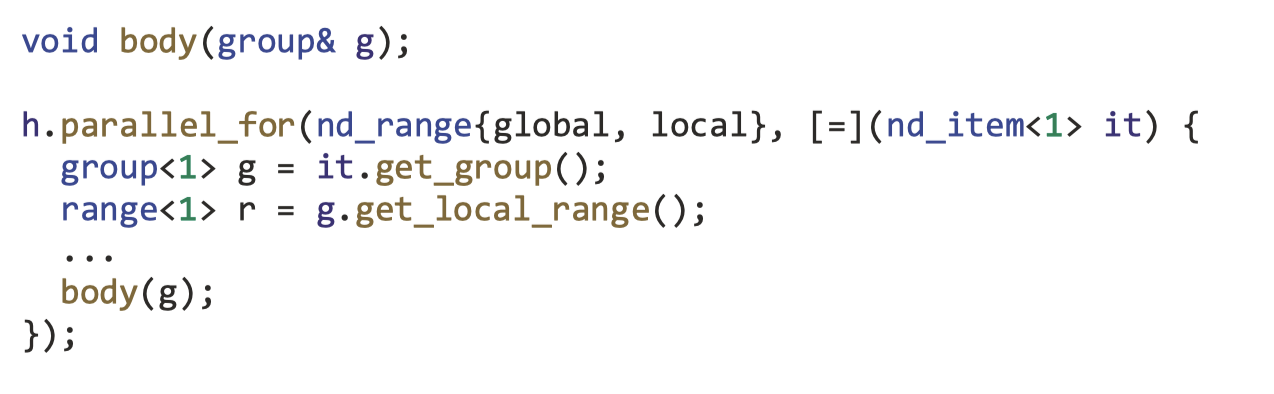
\includegraphics[width=0.9\textwidth]{figs/F4.20.png}
	\caption{\textit{使用 group 类提高可读性}}
\end{figure}

group 类启用的另一个强大选项是能够编写通过模板参数接受任何类型的组的通用组函数。 
尽管 SYCL(尚未)定义正式的 Group“概念”(在 C++20 意义上),
但 group 和 sub\_group 类公开了一个公共接口,允许使用 SYCL::is\_group\_v 等特征来约束模板化 SYCL 函数。 
如今,这种通用编码形式的主要优点是能够支持具有任意维数的Work-Groups,
以及允许函数的调用者决定该函数是否应该在Work-Items之间划分工作的能力。 Work-Groups或Sub-Groups中的Work-Items。 
然而,SYCL 组接口被设计为可扩展的,我们期望在 SYCL 的未来版本中出现更多代表不同Work-Items分组的类。

\paragraph{sub\_group 类}

sub\_group类封装了与Sub-Groups相关的所有功能,简化的定义如图4-21所示。 
与Work-Groups不同,sub\_group 类是访问Sub-Groups功能的唯一方法; 它的功能在 nd\_item 中没有重复。

\begin{figure}[H]
	\centering
	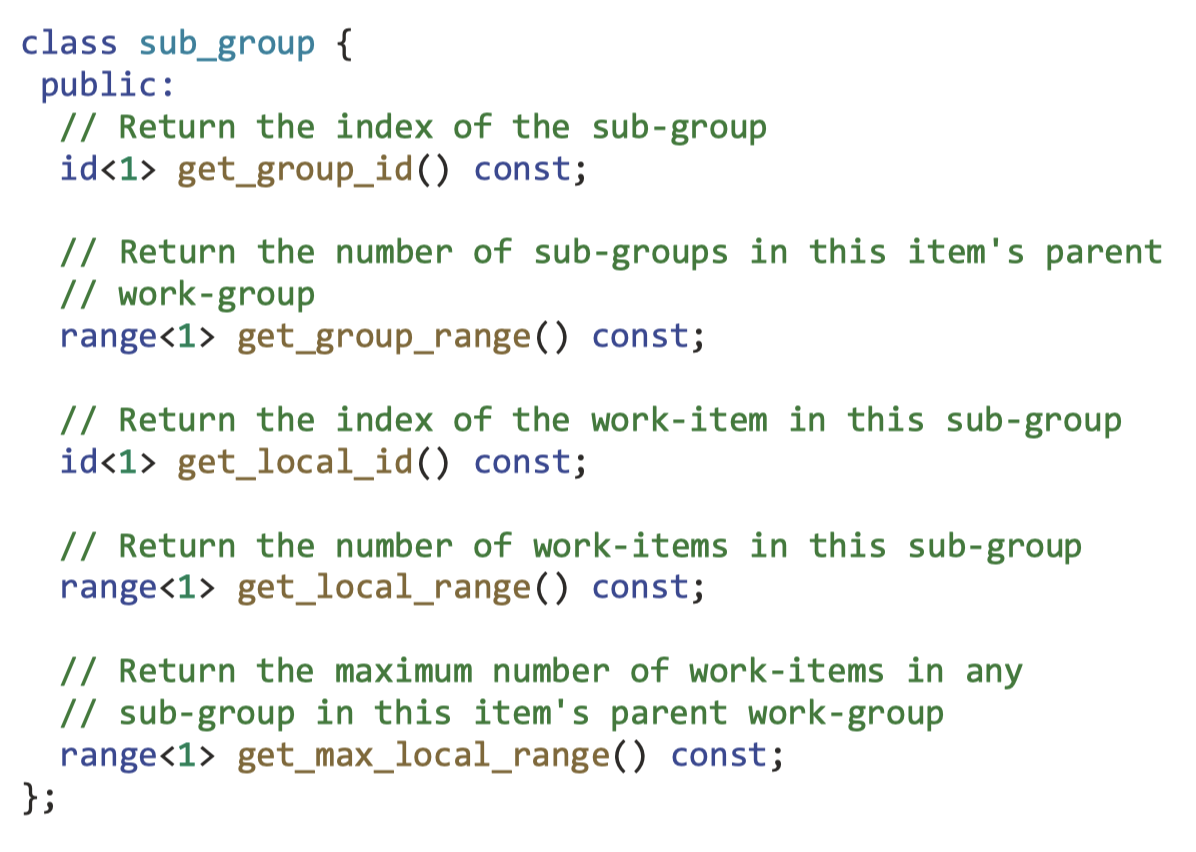
\includegraphics[width=0.9\textwidth]{figs/F4.21.png}
	\caption{\textit{sub\_group 类的简化定义}}
\end{figure}

请注意,有单独的函数用于查询当前Sub-Groups中的Work-Items数以及Work-Groups内任何Sub-Groups中的最大Work-Items数。 
这些是否不同以及如何不同取决于具体设备的Sub-Groups实现方式,
但其目的是反映编译器目标Sub-Groups大小与运行时Sub-Groups大小之间的任何差异。 
例如,非常小的Work-Groups可以包含比编译时Sub-Groups大小更少的Work-Items,
或者可以使用不同大小的Sub-Groups来处理不能被Sub-Groups大小整除的Work-Groups和维度。

\subsection{将计算映射到Work-Items}
到目前为止,大多数代码示例都假设Kernel函数的每个实例对应于对单条数据的单个操作。 
这是一种编写Kernel的简单方法,但这种一对一的映射不是由 SYCL 或任何Kernel形式决定的——
我们始终可以完全控制数据(和计算)分配给各个Work-Items,并且 使该分配可参数化可以是提高性能可移植性的好方法。

\subsubsection{一对一映射}
当我们编写Kernel以实现工作到Work-Items的一对一映射时,这些Kernel必须始终使用范围或 nd\_range 启动,
其大小与需要完成的工作量完全匹配。 这是编写Kernel的最明显的方法,
在许多情况下,它工作得非常好——我们可以相信一个实现可以有效地将Work-Items映射到硬件。

然而,当调整系统和实现的特定组合的性能时,可能需要更加密切地关注低级调度行为。 
Work-Groups对计算资源的调度是实现定义的,并且可能是动态的(即,当计算资源完成一个Work-Groups时,
它执行的下一个Work-Groups可能来自共享队列)。 动态调度对性能的影响并不是固定的,
其重要性取决于Kernel函数每个实例的执行时间以及调度是在软件(例如在CPU上)还是硬件(例如在CPU上)中实现的因素。 
图形处理器)。

\subsubsection{多对一映射}
另一种方法是编写具有工作到Work-Items的多对一映射的Kernel。 
在这种情况下,范围的含义发生了微妙的变化:范围不再描述要完成的工作量,而是描述要使用的工人数量。 
通过更改工人数量和分配给每个工人的工作量,我们可以微调工作分配以最大限度地提高性能。

编写这种形式的Kernel需要进行两处更改:

\begin{enumerate}
	\item Kernel必须接受一个描述工作总量的参数。

	\item Kernel必须包含一个将工作分配给Work-Items的循环。
\end{enumerate}

图 4-22 给出了此类Kernel的一个简单示例。 请注意,Kernel内部的循环有一种稍微不寻常的形式 - 
起始索引是Work-Items在全局范围内的索引,步幅是Work-Items的总数。 
这种数据到Work-Items的循环调度确保循环的所有 N 次迭代都将由Work-Items执行,
而且线性Work-Items访问连续的内存位置(以改进缓存局部性和矢量化行为)。 
工作可以类似地跨组或各个组中的Work-Items进行分配,以进一步改善局部性。

\begin{figure}[H]
	\centering
	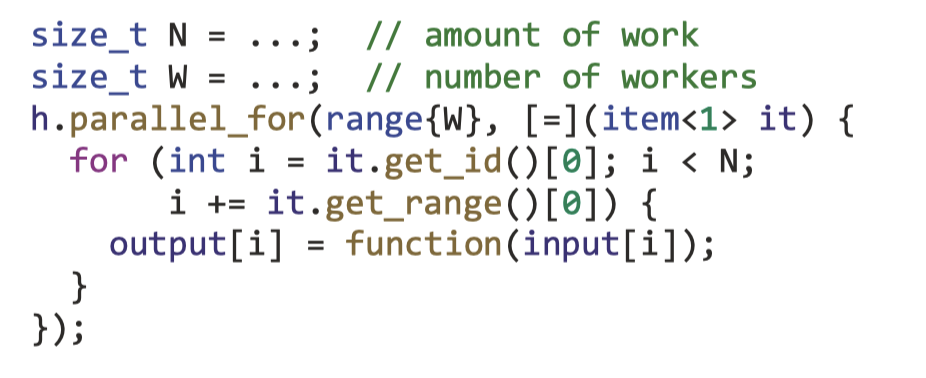
\includegraphics[width=0.9\textwidth]{figs/F4.22.png}
	\caption{\textit{具有独立数据和执行范围的Kernel}}
\end{figure}

这些工作分配模式很常见,我们预计 SYCL 的未来版本将引入语法糖来简化 ND 范围Kernel中工作分配的表达。

\subsection{选择Kernel形式}
在不同的Kernel形式之间进行选择很大程度上取决于个人喜好,并且很大程度上受到其他并行编程模型和语言的先前经验的影响。

选择特定Kernel形式的另一个主要原因是它是公开Kernel所需的某些功能的唯一形式。 
不幸的是,在开发开始之前很难确定需要哪些功能,特别是当我们仍然不熟悉不同的Kernel形式及其与各种类的交互时。

我们根据自己的经验构建了两个指南来帮助我们驾驭这个复杂的空间。 
这些指南应被视为初步建议,绝对不是为了取代我们自己的实验 - 
在不同Kernel形式之间进行选择的最佳方法始终是花一些时间编写每个Kernel形式,
以便了解哪种形式是最好的 适合我们的应用和开发风格。

\begin{figure}[H]
	\centering
	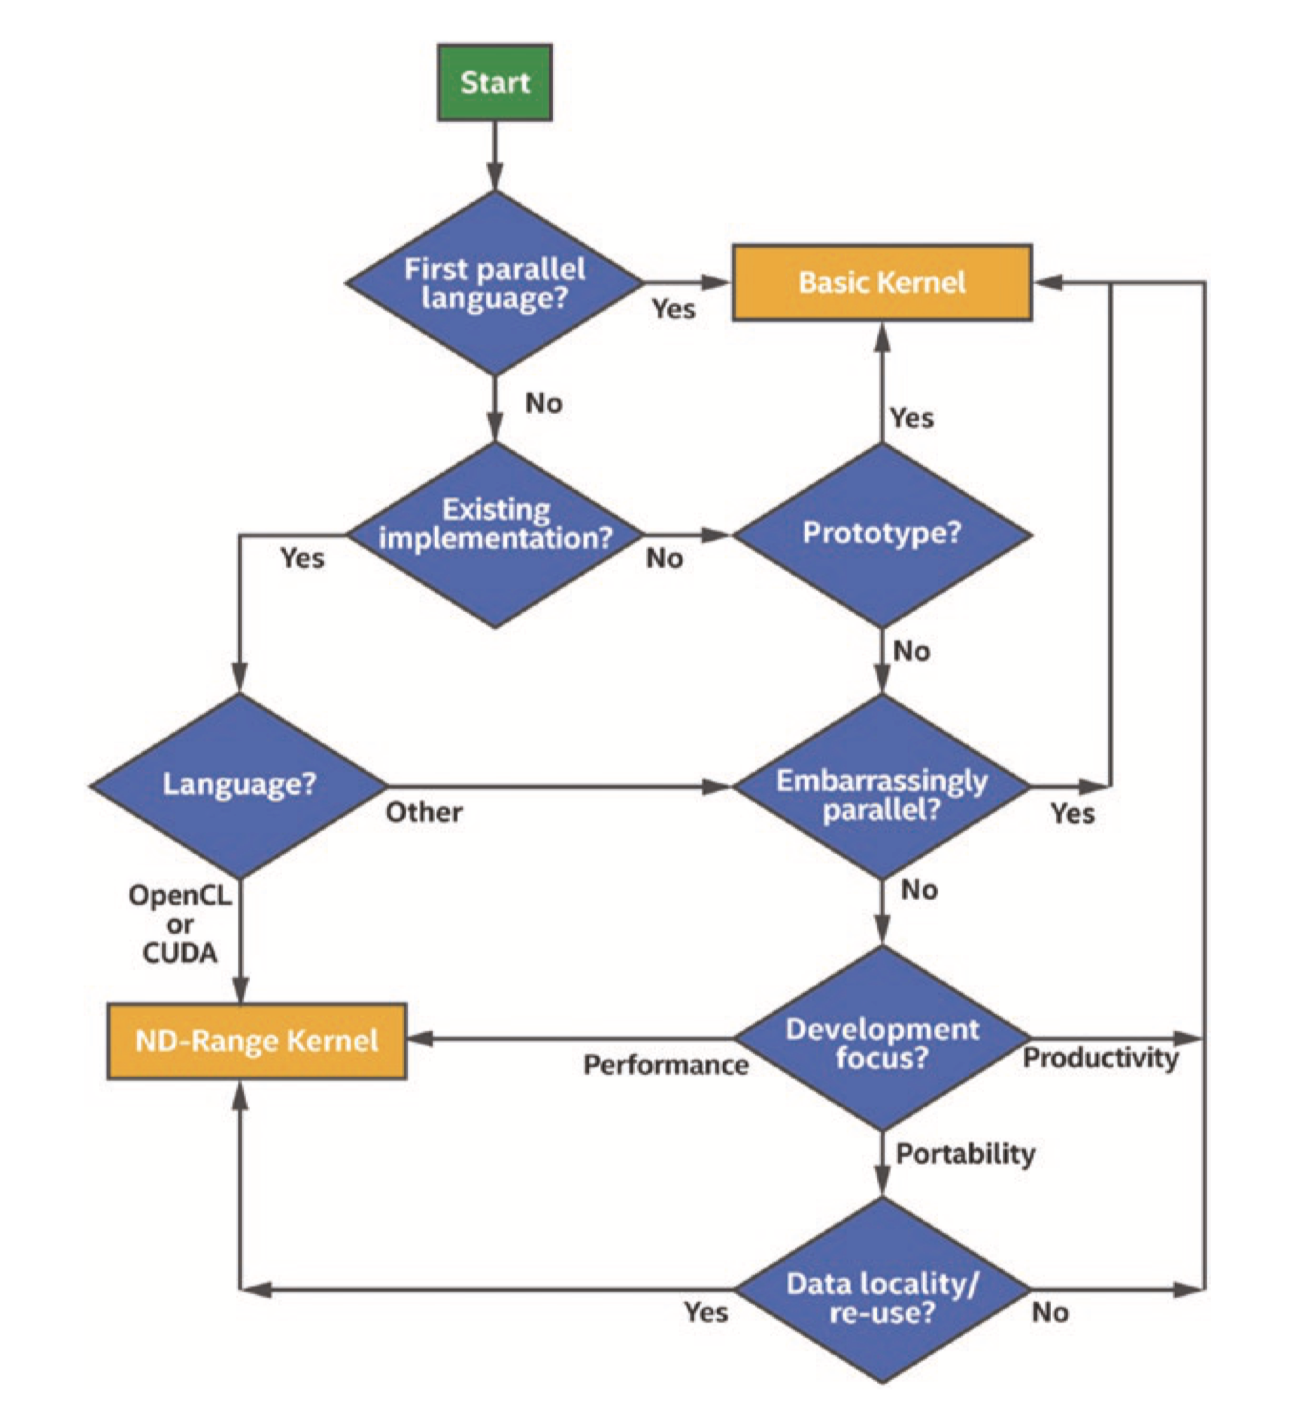
\includegraphics[width=0.9\textwidth]{figs/F4.23.png}
	\caption{\textit{帮助为我们的Kernel选择正确的形式}}
\end{figure}

第一个指南是图4-23所示的流程图,它根据以下条件选择Kernel形式:

\begin{enumerate}
	\item 我们是否有并行编程的经验

	\item 无论我们是从头开始编写新代码还是移植用不同语言编写的现有并行程序

	\item 我们的Kernel是否是高度并行的,或者在Kernel函数的不同实例之间重用数据

	\item 我们是否在 SYCL 中编写新Kernel是为了最大限度地提高性能、提高代码的可移植性,
	还是因为它提供了比低级语言更高效的表达并行性的方法
\end{enumerate}

第二个指南是向每个Kernel形式公开的功能集。 Work-Groups、Sub-Groups、组Barrier、组本地内存、组函数(例如广播)
和组算法(例如扫描、归约)仅适用于 ND-range Kernel,
因此我们应该更喜欢 NDrange Kernel 在我们有兴趣表达复杂算法或微调性能的情况下。

随着语言的发展,每种Kernel形式可用的功能预计会发生变化,
但我们预计基本趋势保持不变:基本数据并行Kernel不会公开局部感知功能,显式 ND 范围Kernel将公开所有性能支持功能 特征。

\subsection{总结}
本章介绍了使用 SYCL 在 C++ 中表达并行性的基础知识,并讨论了每种编写数据并行Kernel的方法的优点和缺点。

SYCL 提供对多种形式的并行性的支持,我们希望我们已经提供了足够的信息来帮助读者做好准备并开始编码!

我们只触及了表面,接下来将更深入地探讨本章中介绍的许多概念和类:第 9 章介绍了本地内存、Barrier和通信例程的使用; 
除了使用 lambda 表达式之外定义Kernel的不同方法将在第 10 章和第 20 章中讨论; 
第 15、16 和 17 章探讨了 ND 范围执行模型到特定硬件的详细映射; 
第 14 章介绍了使用 SYCL 表达常见并行模式的最佳实践。